\documentclass{beamer}

\usepackage{amsmath,amssymb,graphicx}

\usetheme{AAUsimple}

\DeclareMathOperator{\CC}{\mathbb{C}}
\DeclareMathOperator{\cubicDeltaZero}{b^2-3ac}
\DeclareMathOperator{\cubicDeltaOne}{2b^3-9abc+27a^2d}
\DeclareMathOperator{\cubicC}{\sqrt[3]{\frac{\cubicDeltaOne + \sqrt{\left(\cubicDeltaOne\right)^2 - 4\left(\cubicDeltaZero\right)^3}}{2} }}

\makeatletter
\newcommand{\vast}{\bBigg@{4}}
\newcommand{\Vast}{\bBigg@{5}}
\makeatother

%%%%%%%%%%%%%%%%%%%%%%%%%%%%%%%%%%%%%%%%%%%%%%%%%%%%%%%%%%%%%%%%%%%%%%%%%%%%%%%
\title{Smale's Alpha Theory --- Verifying Newton's Method}

\author{
  Chris Swierczewski\\
  {\tt cswiercz@uw.edu}
}

\date{21 January 2016}

\institute{
  Department of Applied Mathematics\\
  University of Washington\\
  Seattle, Washington
}

\pgfdeclareimage[height=1.5cm]{titlepagelogo}{AAUgraphics/aau_logo_new_circle}

\titlegraphic{
  \pgfuseimage{titlepagelogo}
}
%%%%%%%%%%%%%%%%%%%%%%%%%%%%%%%%%%%%%%%%%%%%%%%%%%%%%%%%%%%%%%%%%%%%%%%%%%%%%%%



%%%%%%%%%%%%%%%%%%%%%%%%%%%%%%%%%%%%%%%%%%%%%%%%%%%%%%%%%%%%%%%%%%%%%%%%%%%%%%%
\begin{document}
%%%%%%%%%%%%%%%%%%%%%%%%%%%%%%%%%%%%%%%%%%%%%%%%%%%%%%%%%%%%%%%%%%%%%%%%%%%%%%%

\begin{frame}[plain,noframenumbering]
  \titlepage
\end{frame}


%%%%%%%%%%%%%%%%%%%%%%%%%%%%%%%%%%%%%%%%%%%%%%%%%%%%%%%%%%%%%%%%%%%%%%%%%%%%%%%
\section{Newton's Method For Numerical Approximation}
%%%%%%%%%%%%%%%%%%%%%%%%%%%%%%%%%%%%%%%%%%%%%%%%%%%%%%%%%%%%%%%%%%%%%%%%%%%%%%%


\begin{frame}
  \frametitle{Newton's Method}
  Let $f: \CC \to \CC$ be a polynomial. Define,
  \[
  N(f,x_0)
  =
  \begin{cases}
    x_0 - f(x_0) / f'(x_0) & \text{if } f'(x_0) \neq 0, \\
    x_0 & \text{if } f'(x_0) = 0.
  \end{cases}
  \]
  \pause
  \[
  N^k(f,x_0) =
  \underbrace{(N \circ N \circ \cdots \circ N)}_{k \text{ times}} (f,x_0)
  \]
  \pause
  Convergence
  \[
  \lim_{k \to \infty} N^k(f,x_0) = \xi \text{ a root of $f$}
  \]
\end{frame}

\begin{frame}
  \frametitle{Example}

  \begin{block}{Roots of a Simple Cubic}
    \[
    f(x) = x^3 - 1
    \]
  \end{block}
  Actual roots:
  \[
  \xi_k = e^{2 \pi i k / 3}, \text{for } k = 0,1,2.
  \]
\end{frame}



\begin{frame}
  \frametitle{Example: Actual Roots}
  \begin{figure}
    \centering
    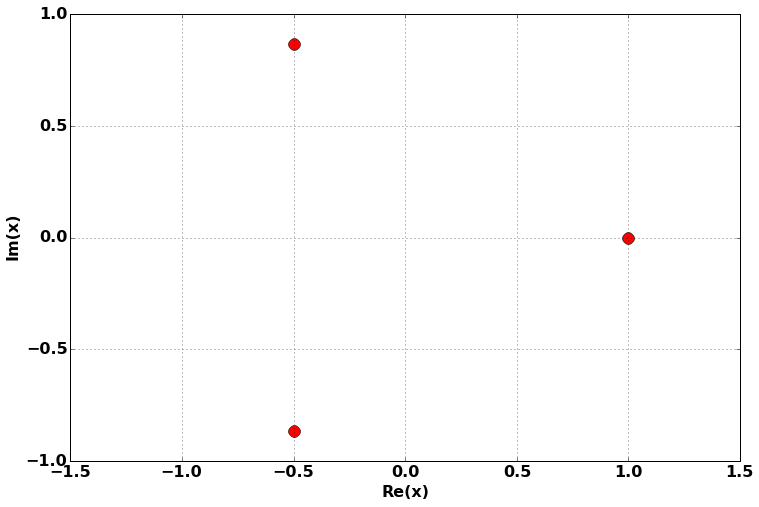
\includegraphics[width=0.95\textwidth]{images/newton_roots.png}
  \end{figure}
\end{frame}



\begin{frame}
  \frametitle{Example: What is a ``Good Guess''?}

  An initial guess ``close'' to the root should converge to that root:

  \pause

  \begin{block}{Next Slide}
  \begin{itemize}
  \item white region $\to$ guesses converging to $\xi_0$,
  \item grey region $\to$ guesses converging to $\xi_1$,
  \item black region $\to$ guesses converging to $\xi_2$,
  \end{itemize}
  \end{block}

  (Apply Newton's Method to each guess until we reach a root.)
\end{frame}




\begin{frame}
  \frametitle{Example: What is a ``Good Guess''?}
  \begin{figure}
    \centering
    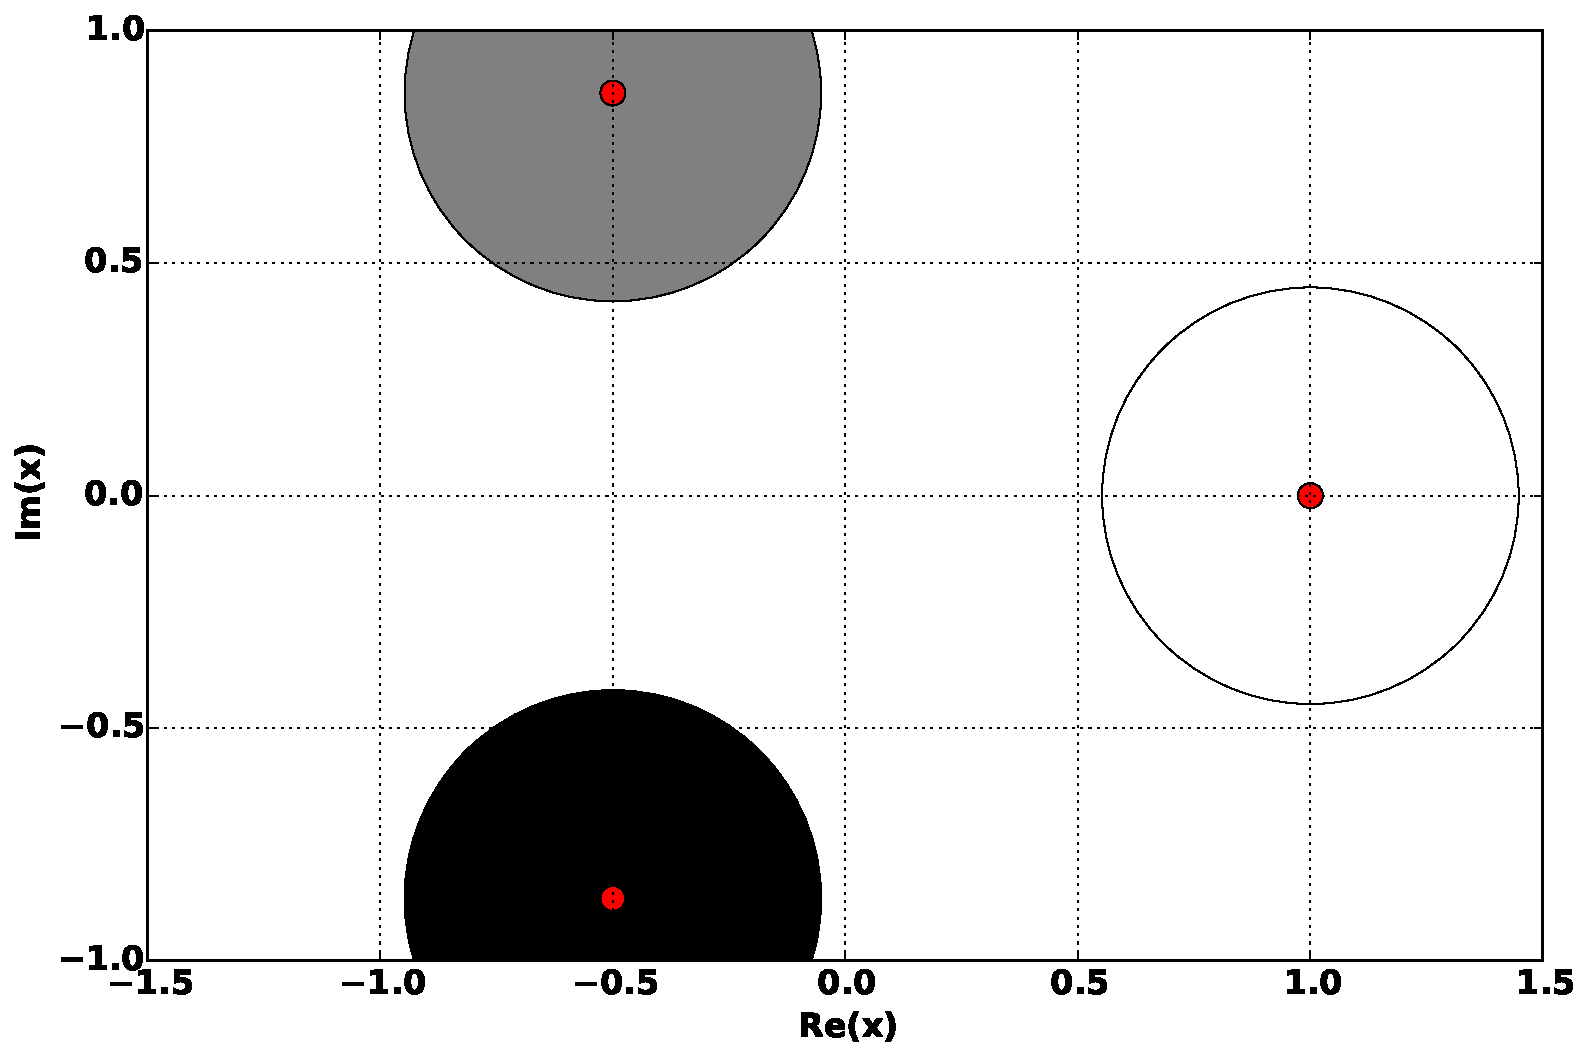
\includegraphics[width=0.95\textwidth]{images/newton_roots_circles.pdf}
  \end{figure}
\end{frame}


\begin{frame}
  \frametitle{Example: What is a ``Bad Guess''?}

  What if the initial Newton guess is further away? \\

  \pause

  \vspace{16pt}

  \begin{block}{Next Slide}
    \begin{itemize}
    \item white region $\to$ guesses converging to $\xi_0$,
    \item grey region $\to$ guesses converging to $\xi_1$,
    \item black region $\to$ guesses converging to $\xi_2$,
  \end{itemize}
  \end{block}

\end{frame}


\begin{frame}
  \frametitle{Example: What is a ``Bad Guess''?}
  \begin{figure}
    \centering
    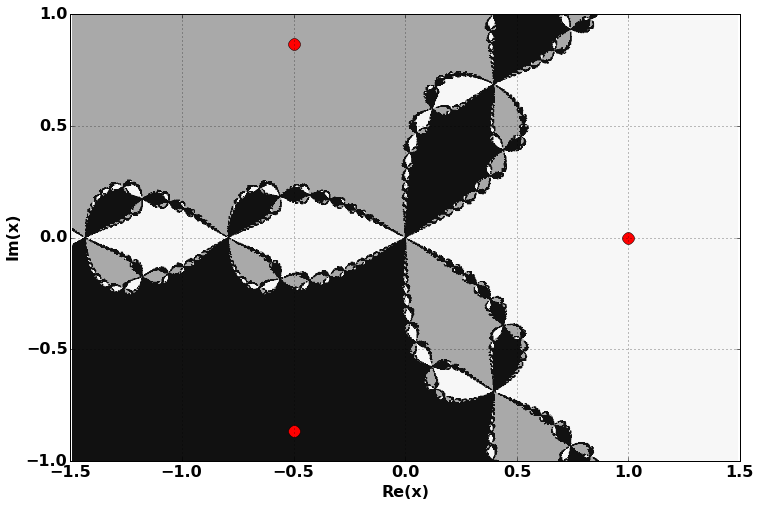
\includegraphics[width=0.95\textwidth]{images/newton.png}
  \end{figure}
\end{frame}




\begin{frame}
  \frametitle{Moral of Story}

  \begin{center}
    {\Huge There are many terrible guesses.}
  \end{center}

  \pause

  \vspace{3cm}

  \begin{center}
    (Even guesses closer to some roots converge to other roots.)
  \end{center}
\end{frame}



\begin{frame}
  \frametitle{Example: Roots of $f(x) = x^9 - 1$}
  \begin{figure}
    \centering
    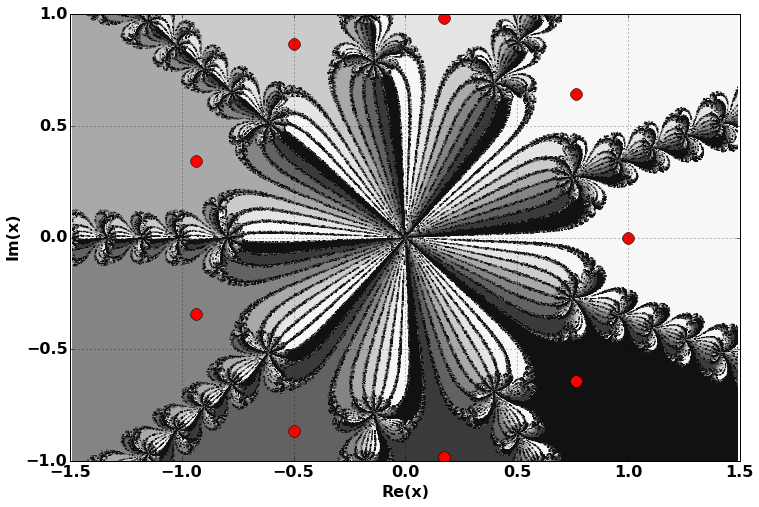
\includegraphics[width=0.95\textwidth]{images/newtonalt.png}
  \end{figure}
\end{frame}



\begin{frame}
  \frametitle{Two Questions}

  \begin{block}{Question \#1}
    Can we ensure our guesses are far away from nasty fractal areas?
  \end{block}

  \pause

  \begin{block}{Question \#2}
    Given two guesses can we determine if they will converge to different roots?
    (Or the same root?)
  \end{block}

  \pause

  \begin{block}{But...}
    ...can we do these a priori? {\it (w/o knowing location of roots)}
  \end{block}

\end{frame}



\begin{frame}
  \frametitle{Terminology}

  Let $f : \CC \to \CC$ be a polynomial.

  \begin{itemize}
  \item<1-> Define: $x \in \CC$ is an {\bf approximate solution} to $f$ with
    {\bf associated solution} $\xi \in \CC$ if

    \[
      \left|N^{(k)}(f,x) - \xi\right|
      \leq
      \left(\tfrac{1}{2}\right)^{2^k-1}
      |x - \xi|
    \]
  \item<2-> approximate solutions converge quadratically to their associated
    soltuions
  \item<3-> {\it ``$x$ lies inside the quadratic convergence region of $\xi$''}
  \end{itemize}
\end{frame}




\begin{frame}
  \frametitle{Quadratic Convergence Region}
  \begin{figure}
    \centering
    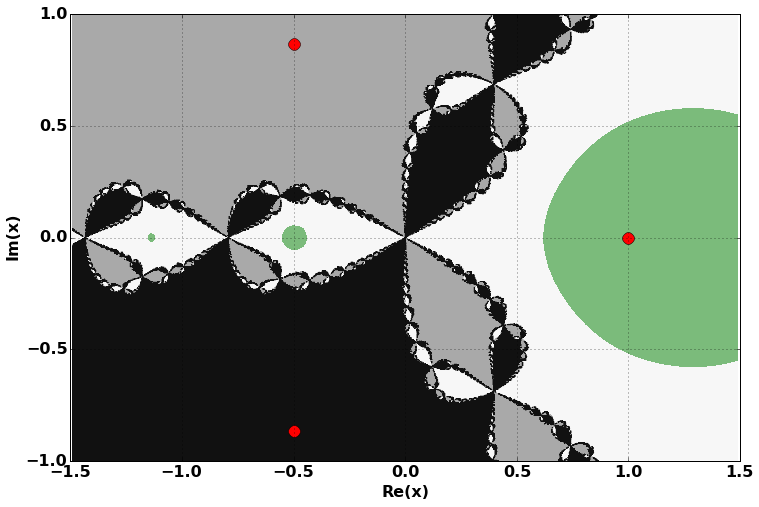
\includegraphics[width=0.9\textwidth]{images/quadratic.png}
    \caption{Quadratic convergence region of $\xi = 1$ for $f(x) =
      x^3-1$.}
  \end{figure}
\end{frame}



\begin{frame}
  \frametitle{Question \#1: Ensuring Quadratic Convergence}

  Determine if $x$ is an {\bf approximate solution}.
  \begin{itemize}
    \item<2-> {\bf Problem}: the condition
      \[
      \left|N^{(k)}(f,x) - \xi\right|
      \leq
      \left(\tfrac{1}{2}\right)^{2^k-1}
      |x - \xi|
      \]
      requires knowing $\xi$!
    \item<3-> {\bf Smale's Alpha Theory}: sufficient conditions for $x$ to be in {\it
        some} quadratic convergence region
  \end{itemize}
\end{frame}



\begin{frame}
  \frametitle{Question \#1: Ensuring Quadratic Convergence}

  {\bf Smale's alpha theory}: let
  \begin{align*}
    \uncover<2->{
      \alpha(f,x) & := \beta(f,x) \gamma(f,x) \\
    }
    \uncover<3->{
      \beta(f,x) & := \left|
      x - N(f,x)
      \right| = \left|
      f(x) / f'(x)
      \right| \\
    }
    \uncover<4->{
      \gamma(f,x) & := \max_{k \geq 2} \left|
      \frac{f^{(k)}(x) / f'(x)}{k!}
      \right|^\frac{1}{k-1}
    }
  \end{align*}
\end{frame}



\begin{frame}
  \frametitle{Question \#1: Converging to a Given Root}

  \begin{block}{Smale Theorem \#1}
    If $f:\CC \to \CC$ is a polynomial and $x \in \CC$ such that
    \[
    \alpha(f,x) \leq \frac{13 - 3\sqrt{17}}{4} \approx 0.157671
    \]
    then $x$ is an {\bf approximate solution} to $f$.

    \pause

    Additionally,
    \[
    |x - \xi| \leq 2\beta(f,x)
    \]
    where $\xi$ is the {\bf associated solution} to $x$.
  \end{block}

\end{frame}



\begin{frame}
  \frametitle{Alpha Region}
  \begin{figure}
    \centering
    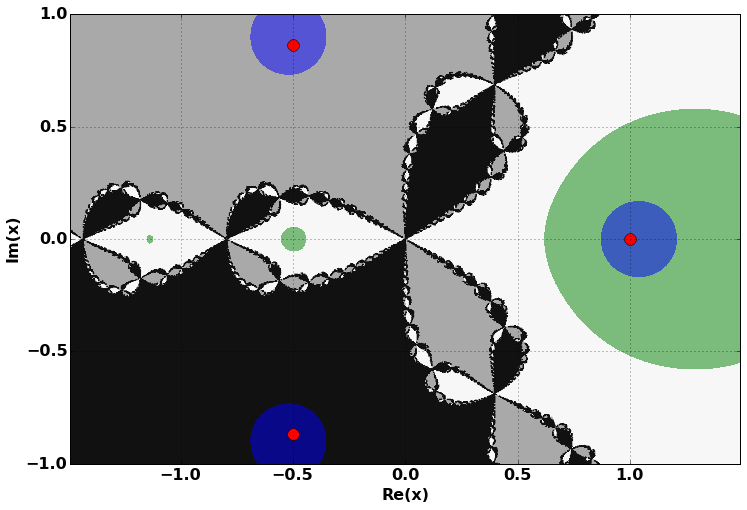
\includegraphics[width=0.9\textwidth]{images/alpha.png}
    \caption{Region where $\alpha(f,x) < 0.157\ldots$ for $f(x) = x^3-1$.}
  \end{figure}
\end{frame}


\begin{frame}
  \frametitle{Alpha Region: Discussion}

  \begin{itemize}
  \item<1-> Pros
    \begin{itemize}
    \item<2-> quadratic convergence condition {\it without} knowing
      roots,
    \item<3-> approximates how far away you are
      \[
      |x - \xi| < 2 \beta(f,x),
      \]
    \end{itemize}
  \item<4-> Cons
    \begin{itemize}
    \item<5-> doesn't say which root (but $\beta$ gives us an idea)
    \item<6-> alpha region much smaller than quad. conv. region
    \end{itemize}
  \end{itemize}
\end{frame}



\begin{frame}
  \frametitle{Question \#2: Converging to Distinct Roots}

  Ensure two {\bf approximate solutions} $x_1, x_2$ have distinct {\bf
    associated solutions} $\xi_1, \xi_2$.

  \pause

  \begin{block}{Smale Theorem \#2}
    If
    \[
    | x_1 - x_2 | > 2 \bigg( \beta(f,x_1) + \beta(f,x_2) \bigg)
    \]
    then
    \[
    \xi_1 \neq \xi_2
    \]
  \end{block}

  \pause

  \begin{itemize}
  \item<3-> Follows from Smale Theorem \#1:
    \[
    | x - \xi | \leq 2 \beta(f,x)
    \]
  \item<4-> {\bf Homework:} prove this
  \end{itemize}

\end{frame}



\begin{frame}
  \frametitle{Application: Analytic Continuation}

  Let $f(x,y) = y^3 - x$.
  \begin{itemize}
  \item<2-> function of $y$ with $x$ as a parameter,
  \item<3-> given an $x$ we can find roots $y_{1},y_{2},y_{3}$ to
    $f(x,y) = 0$,
  \item<4-> {\bf fact:} polynomial roots vary continuously as function of
    coefficients
  \end{itemize}

  \uncover<5->{

  \[
    \text{roots ``above'' } x: \qquad y_1(x),\,y_2(x),\,y_3(x)
  \]

  }

\end{frame}



\begin{frame}
  \frametitle{Example: $f(x,y) = y^3 - x$}
  \begin{columns}
  \begin{column}{0.3\textwidth}
    Let $x_i$ range from $x_0 = 1$ to $x_N = 8$:
    \begin{align*}
    y_1(1)&=1 \\ y_2(1)&=e^{2\pi i/3} \\ y_3(1)&=e^{4\pi i/3} \\ &\vdots \\
    y_1(8)&=2 \\ y_2(8)&=2e^{2\pi i/3} \\ y_3(8)&=2e^{4\pi i/3}
    \end{align*}
  \end{column}

  \begin{column}{0.7\textwidth}
  \begin{figure}
    \centering
    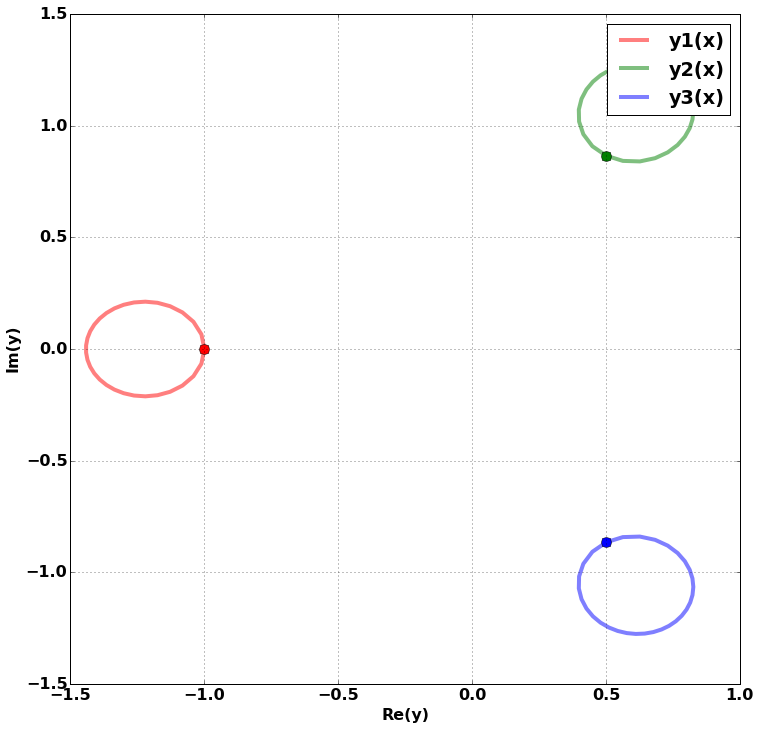
\includegraphics[width=\textwidth]{images/ancontsimple1.png}
  \end{figure}
  \end{column}
  \end{columns}
\end{frame}



\begin{frame}
  \frametitle{Example: $f(x,y) = y^3 - x$}
  \begin{columns}
  \begin{column}{0.3\textwidth}
    Let $x_i$ range along the complex circle
    {\small
    \begin{align*}
      x(t) &= e^{2 \pi i t} - 2 \\
      & t \in [0,1]
    \end{align*}
    }

    \begin{figure}
      \centering
      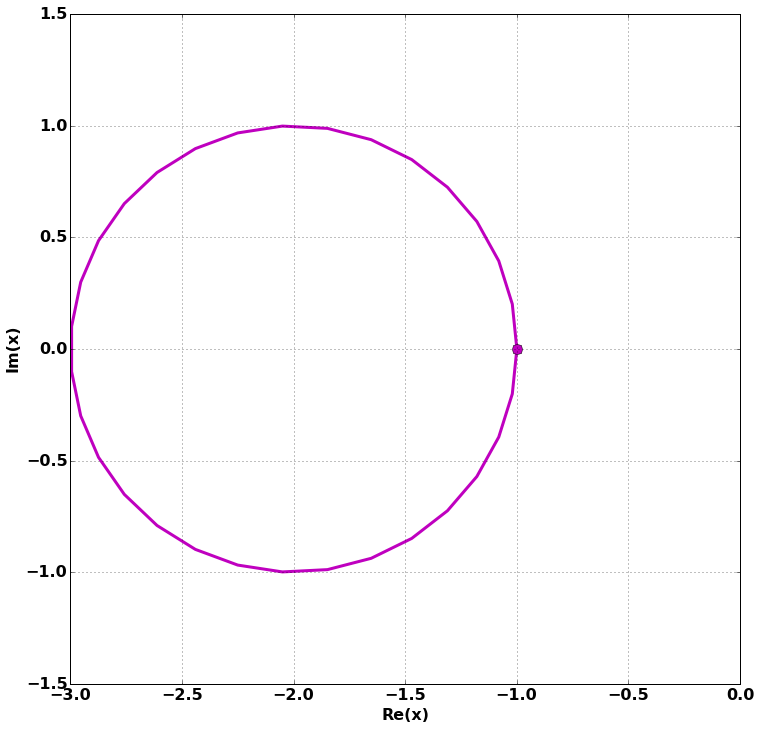
\includegraphics[width=1.2\textwidth]{images/ancontsimplex2.png}
    \end{figure}
  \end{column}

  \begin{column}{0.7\textwidth}
  \begin{figure}
    \centering
    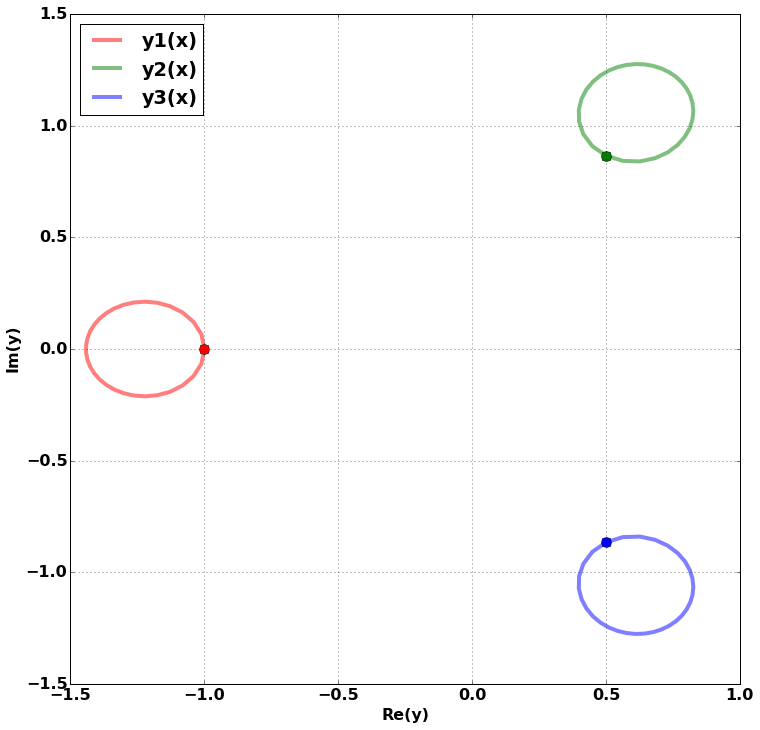
\includegraphics[width=\textwidth]{images/ancontsimple2.png}
  \end{figure}
  \end{column}
  \end{columns}
\end{frame}


\begin{frame}
  \frametitle{Computing These $y$-Paths}

  Let $y_1^{(i)},y_2^{(i)},y_3^{(i)}$ be the $y$-roots computed above
  $x_i$:
  \[
  f(x_i,y) = 0.
  \]

  \pause

  {\bf Goal:} compute corresponding $y$-roots
  \[
  y_1^{(i+1)},y_2^{(i+1)},y_3^{(i+1)}
  \]
  above $x_{i+1}$: {\it solution to $f(x_{i+1},y) = 0$}.

  \begin{itemize}
  \item<3-> {\bf Idea:} use $y_1^{(i)}$ as Newton iteration guess in
    \[
    g(y) := f(x_{i+1}, y) = 0
    \]
    to get $y_1^{(i+1)}$
  \item<4-> {\bf Important:} must satisfy
    \[
    y_1(x_i) = y_1^{(i)} \quad \text{and} \quad y_1(x_{i+1}) = y_1^{(i+1)}
    \]
  \end{itemize}
\end{frame}



\begin{frame}
  \frametitle{Example: $f(x,y) = y^3 - 2x^3y + x^7$}
  \begin{columns}
    \begin{column}{0.3\textwidth}
      Let $x_i$ range along the complex circle
      \begin{align*}
          x(t) &= e^{2 \pi i t} - 2 \\
          & t \in [0,1]
      \end{align*}

      {
        \small {\color{green!60!black} 64 different $x$-values}

        \vspace{16pt}

        {\bf small $\Delta x$ means $y^{(i)}$ are good guesses for $y^{(i+1)}$}

      }

    \end{column}

    \begin{column}{0.7\textwidth}
      \begin{figure}
        \centering
        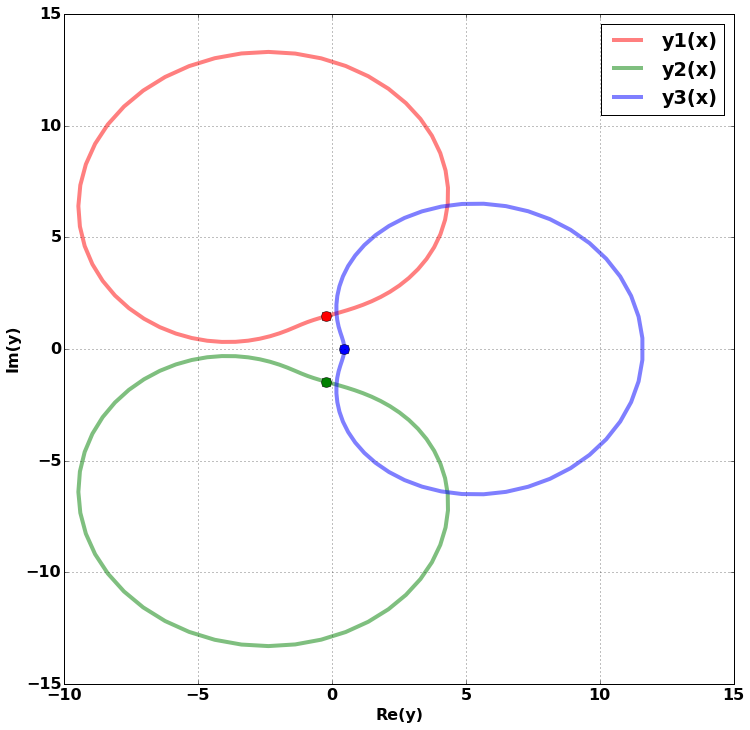
\includegraphics[width=\textwidth]{images/ancontcomplicated64.png}
      \end{figure}
    \end{column}
  \end{columns}
\end{frame}



\begin{frame}
  \frametitle{Example: $f(x,y) = y^3 - 2x^3y + x^7$}
  \begin{columns}
    \begin{column}{0.3\textwidth}
      Let $x_i$ range along the complex circle
      \begin{align*}
          x(t) &= e^{2 \pi i t} - 2 \\
          & t \in [0,1]
      \end{align*}

      {
        \small {\color{red!60!black} 16 different $x$-values}

        \vspace{16pt}

        {\bf Something wrong happened. (Too large $\Delta x$.)} 
      }
    \end{column}

    \begin{column}{0.7\textwidth}
      \begin{figure}
        \centering
        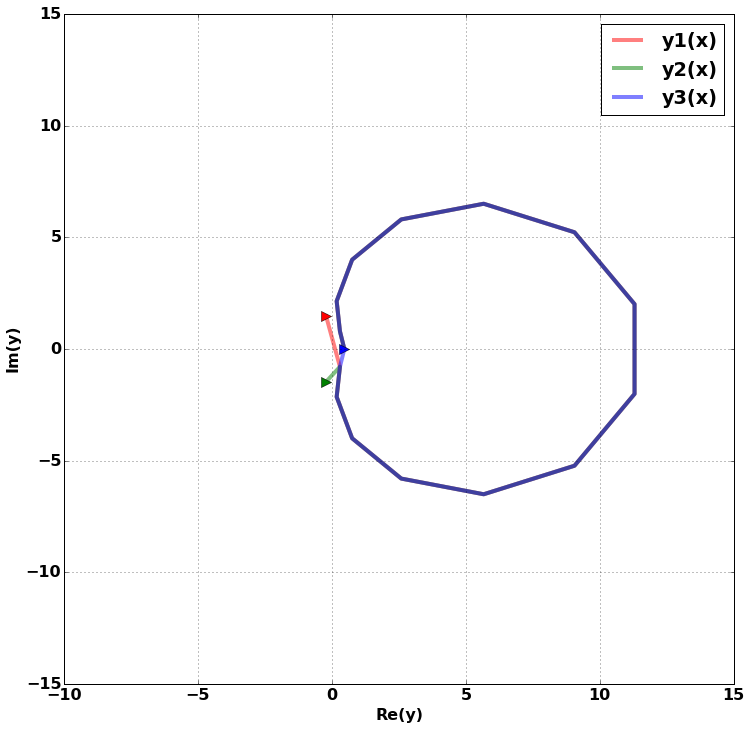
\includegraphics[width=\textwidth]{images/ancontcomplicated16.png}
      \end{figure}
    \end{column}
  \end{columns}
\end{frame}


\begin{frame}
  \frametitle{Problem}

  {\it ``Just take the $\Delta x$ steps to be really small.''}

  \pause

  \vspace{16pt}

  \begin{itemize}
  \item<2-> What does ``small'' mean?
  \item<3-> Heuristics in programming should be avoided. (Understatement of the
    year.)
  \item<4-> Too small $\to$ computationally inefficient.
  \item<5-> {\bf Smale:} determine when $\Delta x$ is small enough such
    that
    \begin{itemize}
    \item<6-> each $y_j^{(i)}$ will converge under Newton \\
      {\bf (Use Smale Theorem \#1)}
    \item<7-> each $y_j^{(i)}$ will converge to {\it distinct}
      $y_j^{(i+1)}$ \\
      {\bf (Use Smale Theorem \#2)}
    \end{itemize}
  \end{itemize}
\end{frame}



\begin{frame}
  \frametitle{Algorithm: Analytic Continutation}

  {\bf Algorithm:} {\tt analytic}$(f,x_i,x_{i+1},y^{(i)})$ \\

  \pause

  {\bf Input:}
  \begin{itemize}
  \item polynomial $f = f(x,y)$,
  \item $x$-points $x_i$ and $x_{i+1}$,
  \item ordered $y$-roots $y^{(i)} = \big( y_1^{(i)}, \ldots, y_d^{(i)}
    \big)$ above $x_i$.
  \end{itemize}

  \pause

  {\bf Output:} ordered $y$-roots $y^{i+1} = \big( y_1^{(i+1)}, \ldots,
  y_d^{(i+1)} \big)$ above $x_{i+1}$.

  \begin{itemize}
    \item such that $y_j^{(i)} \to y_j^{(i+1)}$ (same position $j$)
  \end{itemize}
\end{frame}

\begin{frame}
  \frametitle{Algorithm: Analytic Continutation}

  {\bf Algorithm:} {\tt analytic}$\big(f,\, x_i,\, x_{i+1},\,
  y^{(i)}\big)$ \\

  {\small

  \begin{enumerate}
  \item<1-> Check that each $y_j^{(i)}$ is an {\bf approximate solution} to
    \[
    g(y) := f(x_{i+1},y) = 0
    \]
    using $\alpha(g,y_j^{(i)}) < 0.157\ldots$ If any are not, {\bf refine step}:
    \begin{itemize}
    \item<2-> $x_{i+1/2} \gets (x_i + x_{i+1}) / 2$
    \item<3-> $y^{(i+1/2)} \gets$ {\tt
      analytic}$\big(f,\, x_i, \, x_{i+1/2},\, y^{(i)}\big)$
    \item<4-> $y^{(i+1)} \gets$ {\tt
      analytic}$\big(f,\, x_{i+1/2},\, x_{i+1},\, y^{(i+1/2)}\big)$
    \end{itemize}
  \item<5-> Determine if all {\bf approximate solutions} $y_j^{(i)}$ will
    converge to \underline{distinct} {\bf associated solutions} $y_j^{(i+1)}$:
    \[
    |y_j^{(i)} - y_k^{(i)}| > 2 \big( \beta(f,y_j^{(i)}) +
    \beta(f,y_k^{(i)}) \big), \quad \forall j,k = 1, \ldots, d.
    \]
    If any are not, {\bf refine step}.
  \item<6-> Finally, Newton iterate each $y_j^{(i)}$ to $y_j^{(i+1)}$
    and return.
  \end{enumerate}
  }
\end{frame}




\begin{frame}
  \frametitle{Example: $f(x,y) = y^3 - 2x^3y + x^7$}
  \begin{columns}
    \begin{column}{0.3\textwidth}
      Let $x_i$ range along the complex circle
      \begin{align*}
          x(t) &= e^{2 \pi i t} - 2 \\
          & t \in [0,1]
      \end{align*}

      {
        \small 16 different $x$-values

        \vspace{16pt}

        {\bf Smale guarantees we converge to the correct roots.}
      }

    \end{column}

    \begin{column}{0.7\textwidth}
      \begin{figure}
        \centering
        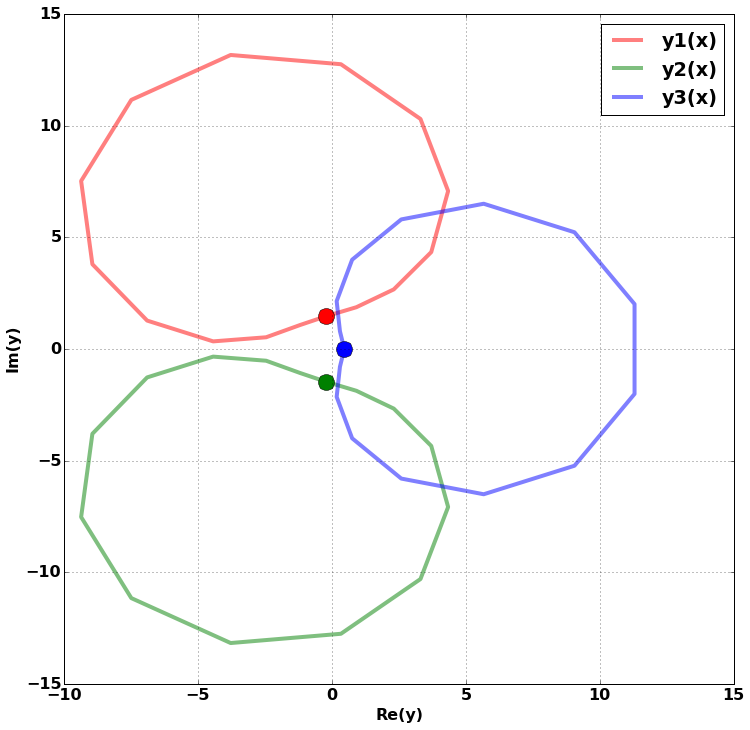
\includegraphics[width=\textwidth]{images/ancontsmale.png}
      \end{figure}
    \end{column}
  \end{columns}
\end{frame}


\begin{frame}
  \frametitle{Example: $f(x,y) = y^3 - 2x^3y + x^7$}
  \begin{columns}
    \begin{column}{0.3\textwidth}
      Let $x_i$ range along the complex circle
      \begin{align*}
          x(t) &= \tfrac{1}{2}e^{2 \pi i t} + \beta \\
          & t \in [0,1]
      \end{align*}
      where
      \[
        \beta \approx -0.8369 - 0.6081j.
      \]
      {\small (Branch point of curve.)}
    \end{column}

    \begin{column}{0.7\textwidth}
      \begin{figure}
        \centering
        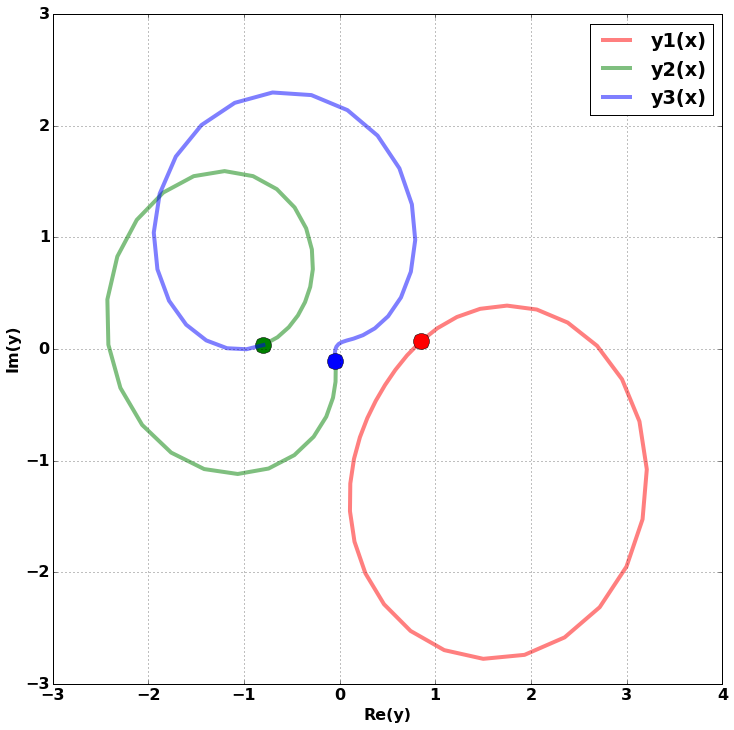
\includegraphics[width=\textwidth]{images/ancontsmalebranch.png}
      \end{figure}
    \end{column}
  \end{columns}
\end{frame}



\begin{frame}
  \frametitle{Final Remarks}

  \begin{itemize}
  \item<1-> Works for square systems of polynomials $f : \CC^n \to
    \CC^n$.
    \begin{itemize}
    \item<2-> Derivative $f' \to$ Jacobian $Df$.
    \end{itemize}
  \item<3-> Even works for smooth functions $f : \CC^n \to \CC^n$.
    \begin{itemize}
    \item<4-> Definition of $\gamma(f,x)$: ``$\max \to \sup$''.
    \item<5-> Some simpler bounds on $\gamma$: results in much smaller
      $\alpha$-region.
    \end{itemize}
  \end{itemize}
\end{frame}



\begin{frame}
  \begin{center}

    \vspace{32pt}

    {\Huge Thank you}

    \vspace{24pt}

    Talk and code available at {\tt www.cswiercz.info}. GitHub repo at {\tt
      github.com/cswiercz/smale}.
  \end{center}

  \vspace{32pt}

  {\tiny
  \begin{block}{References}
    \begin{itemize}
    \item S. Smale, "Newton's method estimates from data at one point", Springer
      New York, 1986.
    \item J. D. Hauenstein, F. Sottile, "AlphaCertified: certifying solutions to
      polynomial systems", ACM Trans. Math. Softw., vol. 38, no. 4, pp. 1-20,
      2012.
    \end{itemize}
  \end{block}
  }
\end{frame}


%%%%%%%%%%%%%%%%%%%%%%%%%%%%%%%%%%%%%%%%%%%%%%%%%%%%%%%%%%%%%%%%%%%%%%%%%%%%%%%
\end{document}
%%%%%%%%%%%%%%%%%%%%%%%%%%%%%%%%%%%%%%%%%%%%%%%%%%%%%%%%%%%%%%%%%%%%%%%%%%%%%%%
